\chapter{Neexpandující impulsní gravitační vlny}
V této kapitole se budeme věnovat neexpandujícím impulsním gravitačním vlnám propagujícím se na pozadí Minkowského a (anti-)de Sitterova
prostoročasu. Popíšeme matematickou konstrukci prostoročasů která vede k tzv. refrakčním rovnícím pro geodetiky, které využijeme k vizualizaci různých
řešení impulsních vln a k interpretaci působení vln na různé testovací částice.


\section{Konstrukce}
Nejprve popíšeme konstrukci prostoročasů s neexpandujícíme impulsními gravitačními vlnami
pomocí Penroseovy geometrické metody \cite{Penrose:1972xrn} "cut and paste", zavedeme souřadnice ve
kterých je metrika spojitá a dále se budeme věnovat distribučnímu popisu prostoročasů s impulsními gravitačními
vlnami.

\subsection{"Cut and paste"\ metoda konstrukce}
\label{sec:cut_and_paste_konstrukce1}
Geometrická metoda konstrukce "cut and paste"\ impulsních gravitačních vln v Minkowského prostoročase \eqref{eq:minkowski} se zakládá na rozdělení celého prostoročasu podél rovinné
světelné nadplochy $\mathcal{N}$, kde je implulzní vlna lokalizována na dvě části $\mathcal{M}^+$ a $\mathcal{M}^-$. Opětovným spojením těchto částí a ztotožněním bodů na hranici
řezu $\mathcal{N}$ se specifickým posunutím dostaneme prostoročas s impulsní gravitační vlnou.

\begin{figure}[ht]\centering
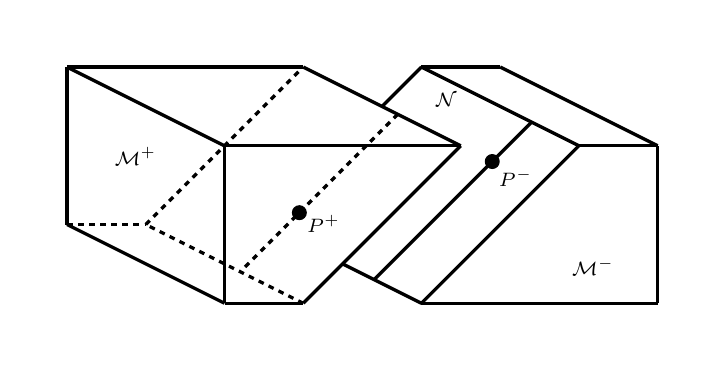
\begin{tikzpicture}
\clip(-2.5,-0.5) rectangle (6.,3.5);
\draw [line width=1.2pt] (-2.,1.)-- (0.,0.);
\draw [line width=1.2pt] (-2.,3.)-- (-2.,1.);
\draw [line width=1.2pt] (0.,0.)-- (0.,2.);
\draw [line width=1.2pt] (0.,2.)-- (-2.,3.);
\draw [line width=1.2pt] (-2.,3.)-- (1.,3.);
\draw [line width=1.2pt] (0.,2.)-- (3.,2.);
\draw [line width=1.2pt] (1.,3.)-- (3.,2.);
\draw [line width=1.2pt] (0.,0.)-- (1.,0.);
\draw [line width=1.2pt] (1.,0.)-- (3.,2.);
\draw [line width=1.2pt,dash pattern=on 2pt off 2pt] (1.,0.)-- (-1.,1.);
\draw [line width=1.2pt,dash pattern=on 2pt off 2pt] (-2.,1.)-- (-1.,1.);
\draw [line width=1.2pt,dash pattern=on 2pt off 2pt] (-1.,1.)-- (1.,3.);
\draw [line width=1.2pt] (2.5,0.)-- (4.5,2.);
\draw [line width=1.2pt] (2.5,0.)-- (5.5,0.);
\draw [line width=1.2pt] (5.5,0.)-- (5.5,2.);
\draw [line width=1.2pt] (4.5,2.)-- (5.5,2.);
\draw [line width=1.2pt] (4.5,2.)-- (2.5,3.);
\draw [line width=1.2pt] (5.5,2.)-- (3.5,3.);
\draw [line width=1.2pt] (2.5,3.)-- (3.5,3.);
\draw [line width=1.2pt] (2.,2.5)-- (2.5,3.);
\draw [line width=1.2pt] (2.5,0.)-- (1.5,0.5);
\draw [line width=1.2pt] (1.9,0.3)-- (3.9,2.3);
\draw [line width=1.2pt,dash pattern=on 2pt off 2pt] (2.2,2.4)-- (0.2,0.4);
\begin{scriptsize}
\draw[color=black] (-1.1302677200189184,1.864045432930641) node {$\mathcal{M}^+$};
\draw[color=black] (2.8186222701156605,2.585603404549911) node {$\mathcal{N}$};
\draw[color=black] (4.6815537604781525,0.46028719723496975) node {$\mathcal{M}^-$};
\draw [fill=black] (0.9503176308657735,1.1503176308657732) circle (2.5pt);
\draw[color=black] (1.2574332042485015,1.0112951028351398) node {$P^+$};
\draw [fill=black] (3.4,1.8) circle (2.5pt);
\draw[color=black] (3.6976110719064135,1.5885414801305562) node {$P^-$};
\end{scriptsize}
\end{tikzpicture}
\caption{Geometrická konstrukce neexpandující impulsní gravitační vlny pomocí metody "cut and paste", 
podél nadplochy $\mathcal{N}$ dojde k rozdělení prostoročasu na dvě části $\mathcal{M}^+$ a $\mathcal{M}^-$ 
a opětovnému ztotožnění bodů na hranici obou částí se specifickým posunem.}
\label{obr01:geomkonstrukt}
\end{figure}

Pro světelnou nadplochu $\mathcal{N}$ danou podmínkou $\mathcal{U}=0$ pak tato konstrukce odpovídá Penroseově 
spojovacím podmínkám

\begin{equation}
    \label{eq:lepici_podminky}
\left[\eta, \bar{\eta}, \mathcal{V}, \mathcal{U}=0_- \right]_{\mathcal{M}^-} \equiv 
\left[\eta, \bar{\eta}, \mathcal{V}-H\left(\eta, \bar{\eta}\right), \mathcal{U}=0_+  \right]_{\mathcal{M}^+},
\end{equation}
kde $H(\eta, \bar{\eta})$ je holomorfní. Penrose \cite{Penrose:1972xrn} ukázal, že impulsní gravitační vlny
jsou v tenzoru křivosti reprezentovány členy proporciálními Diracově delta distribuci $\delta(\mathcal{U})$.
V Minkowského pozadí je nadplocha $\mathcal{U}=0$ rovina a řešení spadá do rodiny impulsních $pp-$vln, tedy
rovnoběžně se propagujících rovinných vln. Obecně na pozadích konstantní křivosti platí stejné napojovací podmínky
\eqref{eq:lepici_podminky} a nadplocha $\mathcal{U}=0$ představuje plochu konstantní Gaussovské křivosti 
$K=\frac{1}{3}\Lambda$ která je popsána metrikou $d\sigma^2=2(1+\frac{1}{6}\Lambda \eta \bar{\eta})^{-2} 
d\eta~d\bar{\eta}$. V případě $\Lambda \neq 0$ se tedy jedná buďto o sféru
($\Lambda > 0$) nebo o hyperbolickou plochu ($\Lambda < 0$). Popis těchto nadploch konstatní křivostsi v (A)dS prostoročasech a
jejich geometrické vlastnosti jsou shrnuty v \cite{Podolsky:1997ri}, kde je také ukázáno,
že se jedná o neexpandující nadplochy.

\begin{figure}[H]
    \centering
    \begin{tikzpicture}
         \node[inner sep=0pt, anchor=south west] (ds) at (0,0)
        {\adjincludegraphics[trim={{.2\width} {.2\height} {.25\width} {.3\height}}, width=.7\textwidth, clip]{../img/kap02/CutAndPaste_NOSUP.pdf}};
        \node[text width=5cm, rotate=45, anchor=north] at (7.6,8.3) {\tiny\textcolor{gray}{$\matu = \pm \infty$}};
        \node[text width=5cm, rotate=45, anchor=north] at (5.6,6.75) {\tiny$\matu = 0$};
    \end{tikzpicture}
    \caption{Nulové geodetiky procházející impulsem nacházejícím se v $\matu=0$ (černá čára) v AdS prostoročase jsou podle cut and paste konstrukce posunuty
    v souřadnici $\matv$ a dochází k refrakci. Geodetiky jsou opět nulovými generátory AdS na $\matu > 0$, neleží už ale v $\eta = 0$ a proto
    neleží na ploše vykresleného hyperboloidu.}
\end{figure}

\subsection{Spojitý tvar metriky}
Metoda "cut and paste"\ nám dává identifikaci bodů prostoročasu na obou stranách impulsní vlny a tedy napojovací podmínky
pro geodetiky, nic ale neříká o podobě metriky kompletního prostoročasu s impulsní vlnou. Potřebujeme tedy najít vhodný
souřadnicový systém, ve kterém bude metrika spojitá funkce $\mathcal{U}$. Toho dosáhneme postupem použitým např. v
\cite{Podolsky:2014ysa}, kde z metriky prostoročasu pozadí \eqref{eq:konfmetric}, respektive
\begin{equation}
    \label{eq:null_background_metric}
    \mathrm{d}s_0^2 = \frac{2~\mathrm{d}\eta~\mathrm{d}\bar{\eta}-2~\mathrm{d}\mathcal{U}~\mathrm{d}\mathcal{V}}
    {\left[1-\frac{1}{6}\Lambda \left(\eta \bar{\eta}
    -\mathcal{U}\mathcal{V}\right)\right]^2},
\end{equation}
souřadnicovou transformací
\begin{equation}
    \label{eq:nonexp_cont_transform}
    \mathcal{U}=U,~~~~ \mathcal{V}=V+H+UH_{,Z}H_{,\bar{Z}},~~~~ \eta=Z+UH_{,\bar{Z}},
\end{equation}
kde uvažujeme libovolnou reálnou funkci $H(Z, \bar{Z})$, obdržíme metriku
\begin{equation}
    \label{eq:nonexp_cont_nokink_metric}
    \mathrm{d} s^{2}=\frac{2\left|\mathrm{d} Z-U\left(H_{, Z \bar{Z}} 
    \mathrm{d} Z+H_{, \bar{Z} \bar{Z}} \mathrm{d} \bar{Z}\right)\right|^{2}-2 \mathrm{d} U 
    \mathrm{d} V}{\left[1-\frac{1}{6} \Lambda(Z \bar{Z}-U V-U G)\right]^{2}}
\end{equation}
kde $G(Z, \bar{Z}) \equiv H - Z H_{,Z}-\bar{Z}H_{,\bar{Z}}$. Metriku \eqref{eq:nonexp_cont_nokink_metric} pak 
uvažujeme pouze pro $U>0$, zatímco na $U<0$ provedeme ztotožnení souřadnic
\begin{equation}
    \label{eq:transformation_just_rename}
    \begin{split}
        &\mathcal{U} = U \\
        &\mathcal{V} = V \\
        &\eta = Z
    \end{split}
\end{equation}
a uvažujeme metriku vzniklou právě touto transformací.
Definováním
tzv. kink funkce jako
\begin{equation}
    \label{eq:kink_function}
    U_+ \equiv U_+(U) = \begin{cases}
        0 & \text{pro } U \leq 0 \\
        U & \text{pro } U \geq 0
    \end{cases}
\end{equation}
můžeme výslednou metriku zapsat jako
\begin{equation}
    \label{eq:nonexp_continuous_metric}
    \mathrm{d} s^{2}=\frac{2\left|\mathrm{d} Z+U_-\left(H_{, Z \bar{Z}} 
    \mathrm{d} Z+H_{, \bar{Z} \bar{Z}} \mathrm{d} \bar{Z}\right)\right|^{2}-2 \mathrm{d} U 
    \mathrm{d} V}{\left[1-\frac{1}{6} \Lambda(Z \bar{Z}-U V-U_+ G)\right]^{2}}.
\end{equation}
Transformace \eqref{eq:nonexp_cont_transform} a \eqref{eq:transformation_just_rename} spojující separátně pro $\mathcal{U}>0$ a $\mathcal{U}<0$ metriku \eqref{eq:null_background_metric}
s metrikou \eqref{eq:nonexp_continuous_metric} lze pomocí Heavisideovy theta funkce $\Theta(U)$ přepsat do tvaru 
\begin{equation}
    \label{eq:nonexp_cont_full_transform}
    \mathcal{U}=U,~~~~ \mathcal{V}=V+\Theta(U) H + U_+ H_{,Z}H_{,\bar{Z}},~~~~ \eta=Z+ U_+ H_{,\bar{Z}}.
\end{equation}
Stále je ale nutné provádět transformaci separátně pro $\mathcal{U}>0$ a $\mathcal{U}<0$, Heavisideova funkce
má při transformaci metriky \eqref{eq:null_background_metric} za následek vznik členů proporcionálních delta funkci. Je také nutné podotknout,
že toto vyjádření je pak ve smyslu distribucí.
Ukazuje se, že tato transformace spojuje tzv. distribuční vyjádření metriky \eqref{eq:nonexp_distr_metric_omega}, které bude zavedeno dále,
se spojitým tvarem metriky \eqref{eq:nonexp_continuous_metric}.
Transformace \eqref{eq:nonexp_cont_full_transform} zároveň obsahuje Penroseovy spojovací podmínky \eqref{eq:lepici_podminky} v $U=0$, kde
vzniká nespojitost v souřadnici $\mathcal{V}$. Tato metoda konstrukce, ve smyslu distribucí, tedy představuje explicitní "cut and paste"\ konstrukci.


\subsection{Distribuční tvar metriky}
Dalším způsobem konstrukce impulsní gravitační vlny je přechod od příslušných rodin tzv. "sandwichových"\
gravtiačních vln s hladkým profilem vlnoplochy k limitnímu distribučnímu vyjádření impulsní vlny. Pro případ neexpandujícíh vln, propagujících se
na $\mathbb{E}^{1,3}$, byl tento limitní přechod uvažován např. v \cite{Penrose1968TwistorQuant}, \cite{Podolsky_1998}, \cite{Podolsky_1998_nonexpanding}.
Výsledná metrika nabývá tvaru
\begin{equation}
    \rmd s^2 = 2~ \rmd \xi \rmd \bar{\xi} - 2 \rmd u \rmd v + H(\xi, \bar{\xi}) \delta\left( u\right) \rmd u^2
\end{equation}

Distribuční tvar metriky také dostaneme dosazením invezní transformace k \eqref{eq:nonexp_cont_full_transform} do spojité metriky 
\eqref{eq:nonexp_continuous_metric}. Vzhledem k nespojitosti v transformaci toto dosazení nemůže být provedeno
v rámci klasické teorie distribucí, kde nelze konzistentně definovat násobení dvou distribucí. S využitím regularizačních metod teorie
nelineárních zobecněných funkcí \textcolor{red}{zde citace}, které zakládají na Colombeaových algebrách, lze ale odvodit pravidla pro násobení
jisté třídy distribucí, která dostačují pro toto odvození. Konkrétně potřebujeme násobit distribuce
\begin{equation}
        \Theta^2 = \Theta, ~~~~ \Theta U_{+} = U_{+}.
\end{equation}
Kromě pravidel pro násobení ještě využijeme identity z klasické teorie distribucí
\begin{equation}
    \Theta' = \delta, ~~~~ U_{+}' = \Theta
\end{equation}
a dostáváme pro libovolnou hodnotu $\Lambda$ metriku ve tvaru
\begin{equation} \label{eq:nonexp_distr_metric_omega}
\mathrm{d}s^2=\frac{2\mathrm{d}\eta~\mathrm{d}\bar{\eta} - 2 \mathrm{d}\mathcal{U}~\mathrm{d}\mathcal{V} + 2H(\eta, \bar{\eta}) \delta(\mathcal{U}) 
~\mathrm{d}\mathcal{U}^2}{\left[1-\frac{1}{6}\Lambda(\eta \bar{\eta}-\mathcal{U}\mathcal{V})\right]^2}.
\end{equation}

V případě nenulové kosmologické konstanty můžeme také využít vnoření do $\mathbb{E}^{1,4}$, případně $\mathbb{E}^{2,4}$ (podle znaménka kosmologické
konstanty, jak je popsáno v kapitole\autoref{chap:kap01}) s dodatečným neexpandujícím impulsem
\begin{equation}
    \label{eq:5DDistributionalWaveMetric}
    \rmd s^2 = \rmd Z_2^2 + \rmd Z_3^2 + \epsilon \rmd Z_4^2 - 2 \rmd \tilde{U} \rmd \tilde{V} + \mathcal{H}(Z_2, Z_3, Z_4) \delta(\tilde{U}) \rmd \tilde{U}^2,
\end{equation}
kde $\epsilon = \text{sign} (\Lambda)$, $\tilde{U} = \tfrac{1}{\sqrt{2}}(Z_0 - Z_1)$, $\tilde{V}= \tfrac{1}{\sqrt{2}}(Z_0 + Z_1)$.
S podmínkou analogickou k \eqref{eq:dS_hyperboloid} a \eqref{eq:AdS_hyperboloid},
\begin{equation}
    Z_2^2 + Z_3^2 + \epsilon Z_4^2 - 2 \tilde{U} \tilde{V} = \epsilon a^2,
\end{equation}
dostáváme reprezentaci impulsních vln propagujících se na (A)dS prostoročasu s impulsem na $\tilde{U}=0$. 
Funkce $H$ a $\mathcal{H}$ v metrikách \eqref{eq:nonexp_distr_metric_omega} a \eqref{eq:5DDistributionalWaveMetric} jsou svázány vztahem
\begin{equation}
    \mathcal{H} = \frac{2H}{1-\frac{1}{6}\Lambda \eta \bar{\eta}}
\end{equation}

\subsection{$\mathcal{C}^1$-matching a refrakční rovnice}
Dále budeme explicitně modelovat geodetiky na prostoročasech s neexpandujícími impulsními vlnami v souřadnicích
\eqref{eq:nonexp_distr_metric_omega}. V těchto souřadnicích není řešení rovnice geodetiky dobře definované v
klasické teorii distribucí, pro neexpandující impulsní vlny na Minkowského prostoročasu byla rovnice geodetiky
a její řešení zkoumána v rámci teorie zobecněných funkcí ve smyslu Colombeaových algeber a v článích \cite{Steinbauer_1998} a \cite{Kunzinger_1999}
byla ukázána existence a jednoznačnost řešení v prostoru těchto funkcí a bylo ověřeno, že geodetiky na $\mathcal{M}^-$ a $\mathcal{M}^+$ odpovídají
geodetikám na Minkowského pozadí se skokem v souřadnici $\matv$ při přechodu přes nadplochu $\matu=0$. V prostoročasech s
nenulovou kosmologickou konstantou lze využít přístup vnoření do pětidimenzionálního Minkowského prostoru, kde se v rovnici
geodetiky nenachází výrazy nedefinované v klasické teorii distribucí, \textcolor{red}{Chápu to tak správně?} řešení rovnice geodetiky
pro (anti-)de Sitterův prostoročas s impulsními neexpandujícími vlnami byly tímto způsobem odvozeny v \cite{Podolsk__2001}.
V článku \cite{Podolsky:2014ysa} byla odvozena rovnice geodetiky v souřadnicích \eqref{eq:nonexp_continuous_metric}.
Odvozený tvar je v tomto případě ve smyslu Filippových řešení (diferenciálních inkluzí) \cite{filippov1988differential}, což je zobecnění teorie obyčejných diferenciálních rovnic.
V článku je ukázána existence a jednoznačnost takových řešení, dále autoři využívají metodou $\mathcal{C}^1$-matchingu,
kde při splnění určitých předpokladů na metriku, lze řešení ve smyslu Filippova přiřadit řešením rovnice geodetiky na jednotlivých částech prostoročasu
("před a za impulsem"), bez nutné znalosti detailů teorie za Filippovými řešeními.

Výsledkem $\mathcal{C}^1$-matchingu je sada refrakčních rovnic, které udávají jak skok v souřadnici $\matv$,
tak i změnu v rychlostech před a za impulsem. Geodetiku procházející impulsní plochou ve spojitých souřadnicích tedy
ztotožníme transformací \eqref{eq:nonexp_cont_full_transform} (a její derivací), v oblastech $U > 0$ a $U < 0$ separátně, s geodetikami v souřadnicích prostoročasu na pozadí.
Pro polohy dostáváme limitou $U \to 0^+$ a $U \to 0^-$ rovnice
\begin{equation}
    \label{eq_refraction_nonexpanding_positions}
    \begin{split}
        \matu^{+}_{\mathrm{i}} &= \matu^{-}_{\mathrm{i}} = 0,\\
        \matv^{+}_{\mathrm{i}} &= \matv^{-}_{\mathrm{i}} + H_{\mathrm{i}},\\
        \eta^{+}_{\mathrm{i}} &= \eta^{-}_{\mathrm{i}},
    \end{split}
\end{equation}
což odpovídá Penroseovým spojovacím podmínkám - geodetika je spojitá v $\matu$ a $\eta$ a dochází ke skoku ve $\matv$.
Pro rychlosti obdržíme stejnou limitou rovnice
\begin{equation}
    \label{eq:refraction_nonexpanding_velocities}
    \begin{split}
        &\dot{\mathcal{U}}^{+}_{\mathrm{i}} = \dot{\mathcal{U}}^{-}_{\mathrm{i}}\\
        &\dot{\mathcal{V}}^{+}_{\mathrm{i}} = \dot{\mathcal{V}}_{\mathrm{i}}^{-} + H_{\mathrm{i}, Z}
        \dot{\eta}^{-}_{\mathrm{i}} + H_{\mathrm{i}, \bar{Z}} \dot{\overline{\eta}}^{-}_{\mathrm{i}} + 
        H_{\mathrm{i}, Z} H_{\mathrm{i}, \bar{Z}} \dot{\mathcal{U}}_{\mathrm{i}}^{-}\\
        &\dot{\eta}_{\mathrm{i}}^{+} =\dot{\eta}_{\mathrm{i}}^{-}+H_{\mathrm{i}, \bar{Z}}
        \dot{\mathcal{U}}_{\mathrm{i}}^{-}.
    \end{split}
\end{equation}
Index $i$ znamená hodnotu na impulsní nadploše $\matu = 0$, složky označené znakem + jsou za impulsem ($\matu > 0$),
složky označené znakem - jsou před impulsem ($\matu <0$).

Všimněme si, že při přechodu přes impulsní plochu platí $\eta_{\mathrm{i}} = Z_{\mathrm{i}}$ a tedy $ H_{\mathrm{i},Z} = \frac{\partial}{\partial \eta} H(\eta, \bar{\eta})$.

Bližším pohledem na refrakční rovnice také vidíme, že zachovávají kauzální charakter. Složka rychlosti $\dot \matu$ se
nemění, ve složkách $\dot \matv$ a $\dot \eta$ dojde k refrakci tak, že nedochází ke změně normy čtyřrychlosti.

Dále ještě uvedeme refrakční rovnice v reálných polárních prostorových souřadnicích, které odvodíme z transformace spojitých souřadnic
$\rho = \sqrt{2} \left|Z + U_{+} H_{,\bar{Z}}\right|$ a $\varphi = \frac{1}{2i} \log \frac{Z + U_+ H_{,\bar{Z}}}{\bar{Z} + U_+ H_{,Z}}$.
Limitou $U \to 0^+$ a $U \to 0^-$ dostáváme
\begin{equation}
    \begin{split}
        \matv^{+}_{\mathrm{i}} &= \matv^{-}_{\mathrm{i}} + H_{\mathrm{i}},\\
        \rho^{+}_{\mathrm{i}} &= \rho^{-}_{\mathrm{i}}\\
        \varphi^{+}_{\mathrm{i}} &= \varphi^{-}_{\mathrm{i}},
    \end{split}
\end{equation}
tedy radiální i úhlová složka jsou spojité. Pro složky rychlosti pak provedeme stejnou limitu na derivaci souřadnic,
\begin{equation}
    \begin{split}
        \dot{\mathcal{V}}_{\mathrm{i}}^{+}=& ~\dot{\mathcal{V}}_{\mathrm{i}}^{-}+\frac{1}{\sqrt{2}}\left(e^{i \varphi_{\mathrm{i}}^{-}} H_{\mathrm{i}, Z}+e^{-i \varphi_{\mathrm{i}}^{-}} H_{\mathrm{i}, \bar{Z}}\right) \dot{\rho}_{\mathrm{i}}^{-}+\frac{i}{\sqrt{2}}\left(e^{i \varphi_{\mathrm{i}}^{-}} H_{\mathrm{i}, Z}-e^{-i \varphi_{\mathrm{i}}^{-}} H_{\mathrm{i}, \bar{Z}}\right) \rho_{\mathrm{i}}^{-} \dot{\varphi}_{\mathrm{i}}^{-} \\
        &+\left(H_{\mathrm{i}, Z} H_{\mathrm{i}, \bar{Z}}\right) \dot{\mathcal{U}}_{\mathrm{i}}^{-} \\
        \dot{\rho}_{\mathrm{i}}^{+}=& \dot{\rho}_{\mathrm{i}}^{+} + \frac{1}{2} \left(e^{i \varphi^-_\mathrm{i}} H_{\mathrm{i},Z} + e^{-i \varphi^-_\mathrm{i}} H_{\mathrm{i},\bar{Z}}\right)\dot{\matu}_\mathrm{i}^{-}\\
        \dot{\varphi}_{\mathrm{i}}^{+}=&\dot{\varphi}_{\mathrm{i}}^{-} + \frac{i}{\sqrt{2}\rho_{\mathrm{i}}^{-}} \left(e^{i \varphi_{\mathrm{i}}^{-}} H_{\mathrm{i}, Z} - e^{-i \varphi_{\mathrm{i}}^{-}} H_{\mathrm{i}, \bar{Z}}\right) \dot{\matu}_{\mathrm{i}}^{-}.
        \end{split}
\end{equation}


Díky tomu, že odvození proběhlo v konformně plochých souřadnicích, nezávisí na hodnotě $\Lambda$ a máme jednotné rovnice pro
refrakci způsobenou impulsními vlnami, propagujícími se v Minkowského i (anti-)de Sitterově prostoročase.

V (anti-)de Sitterově prostoročasech můžeme také využít pětidimenzionálního formalismu a odvodit refrakční rovnice v souřadnicích \eqref{eq:5DDistributionalWaveMetric}.
Konformní faktor je na jednotlivých částech prostoročasu při cut and paste konstrukci daný jako $\Omega^{\pm}_{\mathrm{i}} = 1 + \frac{1}{6} \Lambda \eta^{\pm} \bar{\eta}^{\pm}$,
ze spojitosti $\eta, \bar{\eta}$ při přechodu přes $\matu=0$
však plyne, že pro konformní faktor stačí psát $\Omega_{\mathrm{i}}$, jelikož při přechodu přes impulsní nadplochu nedochází k jeho změně.

Použitím rovnic pro polohy \eqref{eq_refraction_nonexpanding_positions} dostáváme
\begin{align}
        \tilde{U}^{+}_\mathrm{i} &= 0 = \tilde{U}^{-}_\mathrm{i}, &
        \tilde{V}^{+}_\mathrm{i} &= \tilde{V}^{-}_\mathrm{i} + \frac{H_\mathrm{i}}{\Omega_\mathrm{i}}, &
        Z^{+}_{2\mathrm{i}} &= Z^{-}_{2\mathrm{i}}, &
        Z^{+}_{3\mathrm{i}} &= Z^{-}_{3\mathrm{i}}, &
        Z^{+}_{4\mathrm{i}} &= Z^{-}_{4\mathrm{i}}.  &
\end{align}


\textcolor{red}{5dim formalismus!}

\subsection{Vizualizace geodetik prostoročasů s neexpandující impulsní vlnou}
Refrakční rovnice jsou vhodným nástrojem k vizualizaci geodetik v souřadnicích prostoročasů na pozadí impulsní vlny.
Pro vybrané funkce $H$, resp. $\mathcal{H}$ v prostoročasech s $\Lambda \neq 0$, byly zvolené geodetiky před impulsem ztotožněny
s geodetikami za impulsem. Integrací rovnice geodetiky na oblastech před a za impulsem zvlášť pak obdržíme celé geodetiky v prostoročasu s
impulsní vlnou. Pro účel vizualizace geodetik v těchto prostoročasech autor této práce vytvořil balíček GRImpulsiveWaves pro jazyk Python,
tento open-source balíček je volně dostupný na platformě GitHub. \textcolor{red}{přidat na pip!} V následujících podsekcích
představíme vizualizace pro tato vybraná řešení, pro různé parametry a počáteční podmínky geodetik.

\subsection{Impulsní gravitační vlna generovaná nehmotnými částicemi s multipólovou strukturou s $\Lambda=0$}

Řešení impulsní vlny generované nulovými částicemi s multipólovou strukturou v Minkowského prostoročase odvodili
Griffiths a Podolský v \cite{Griffiths_1997}. Polní rovnice se pro tento případ redukují na

\begin{equation}
    \label{eq:podminka_na_H}
    \Delta H = 2 H_{,\eta \bar{\eta}} = 8 \pi T_{\matu \matu},
\end{equation}
 
kde $T_{\matu \matu} = f(\eta, \bar{\eta}) \delta(\matu)$. Funkce $H$ v cylindrických prostorových souřadnicích nabývá tvaru 
\begin{equation}
    \label{eq:multipole_minkowski}
    H = -b_0 \log(\rho) + \sum_{m=1}^\infty b_m \rho^{-m} \cos\left[ m \left(\phi - \phi_m \right) \right],
\end{equation}
kde $b_m$, $\phi_m$ jsou konstanty.

Řešení s jedinou monopólovou částicí, tedy $b_m=0$ pro všechna $m \geq 1$, odpovídá Aichelburg-Sexlovu řešení - prostoročasu
zkonstruovanému ultraboostem Schwarzschildova řešení \cite{Aichelburg_1971}.

\begin{figure}[h]
    \centering
    \begin{subfigure}[b]{0.31\textwidth}
        \begin{tikzpicture}
            \node[inner sep=0pt, anchor=south west] (ds) at (0,0)
           {\adjincludegraphics[trim={{.1\width} {.05\height} {.1\width} {.1\height}}, width=0.9\textwidth, clip]{../img/kap02/monopole.pdf}};
       \end{tikzpicture}
       \caption{}
    \end{subfigure}
     \hfill
     \begin{subfigure}[b]{0.31\textwidth}
        \begin{tikzpicture}
            \node[inner sep=0pt, anchor=south west] (ds) at (0,0)
           {\adjincludegraphics[trim={{.1\width} {.15\height} {.1\width} {.1\height}}, width=\textwidth, clip]{../img/kap02/dipole.pdf}};
       \end{tikzpicture}
       \caption{}
     \end{subfigure}
     \hfill
     \begin{subfigure}[b]{0.31\textwidth}
        \begin{tikzpicture}
            \node[inner sep=0pt, anchor=south west] (ds) at (0,0)
           {\adjincludegraphics[trim={{.1\width} {.18\height} {.1\width} {.1\height}}, width=0.8\textwidth, clip]{../img/kap02/quadrupole.pdf}};
       \end{tikzpicture}
       \caption{}
     \end{subfigure}

    \caption{Funkce $H$ v případě (a) Aichelburg-Sexlova řešní, impulsní vlny generované nulovou částicí s (b) dipólovou strukturou a s (c) kvadrupólovou strukturou}
\end{figure}

\begin{figure}[h]
    \centering
    \begin{tikzpicture}
        \node[inner sep=0pt, anchor=south west] (ds) at (0,0)
        {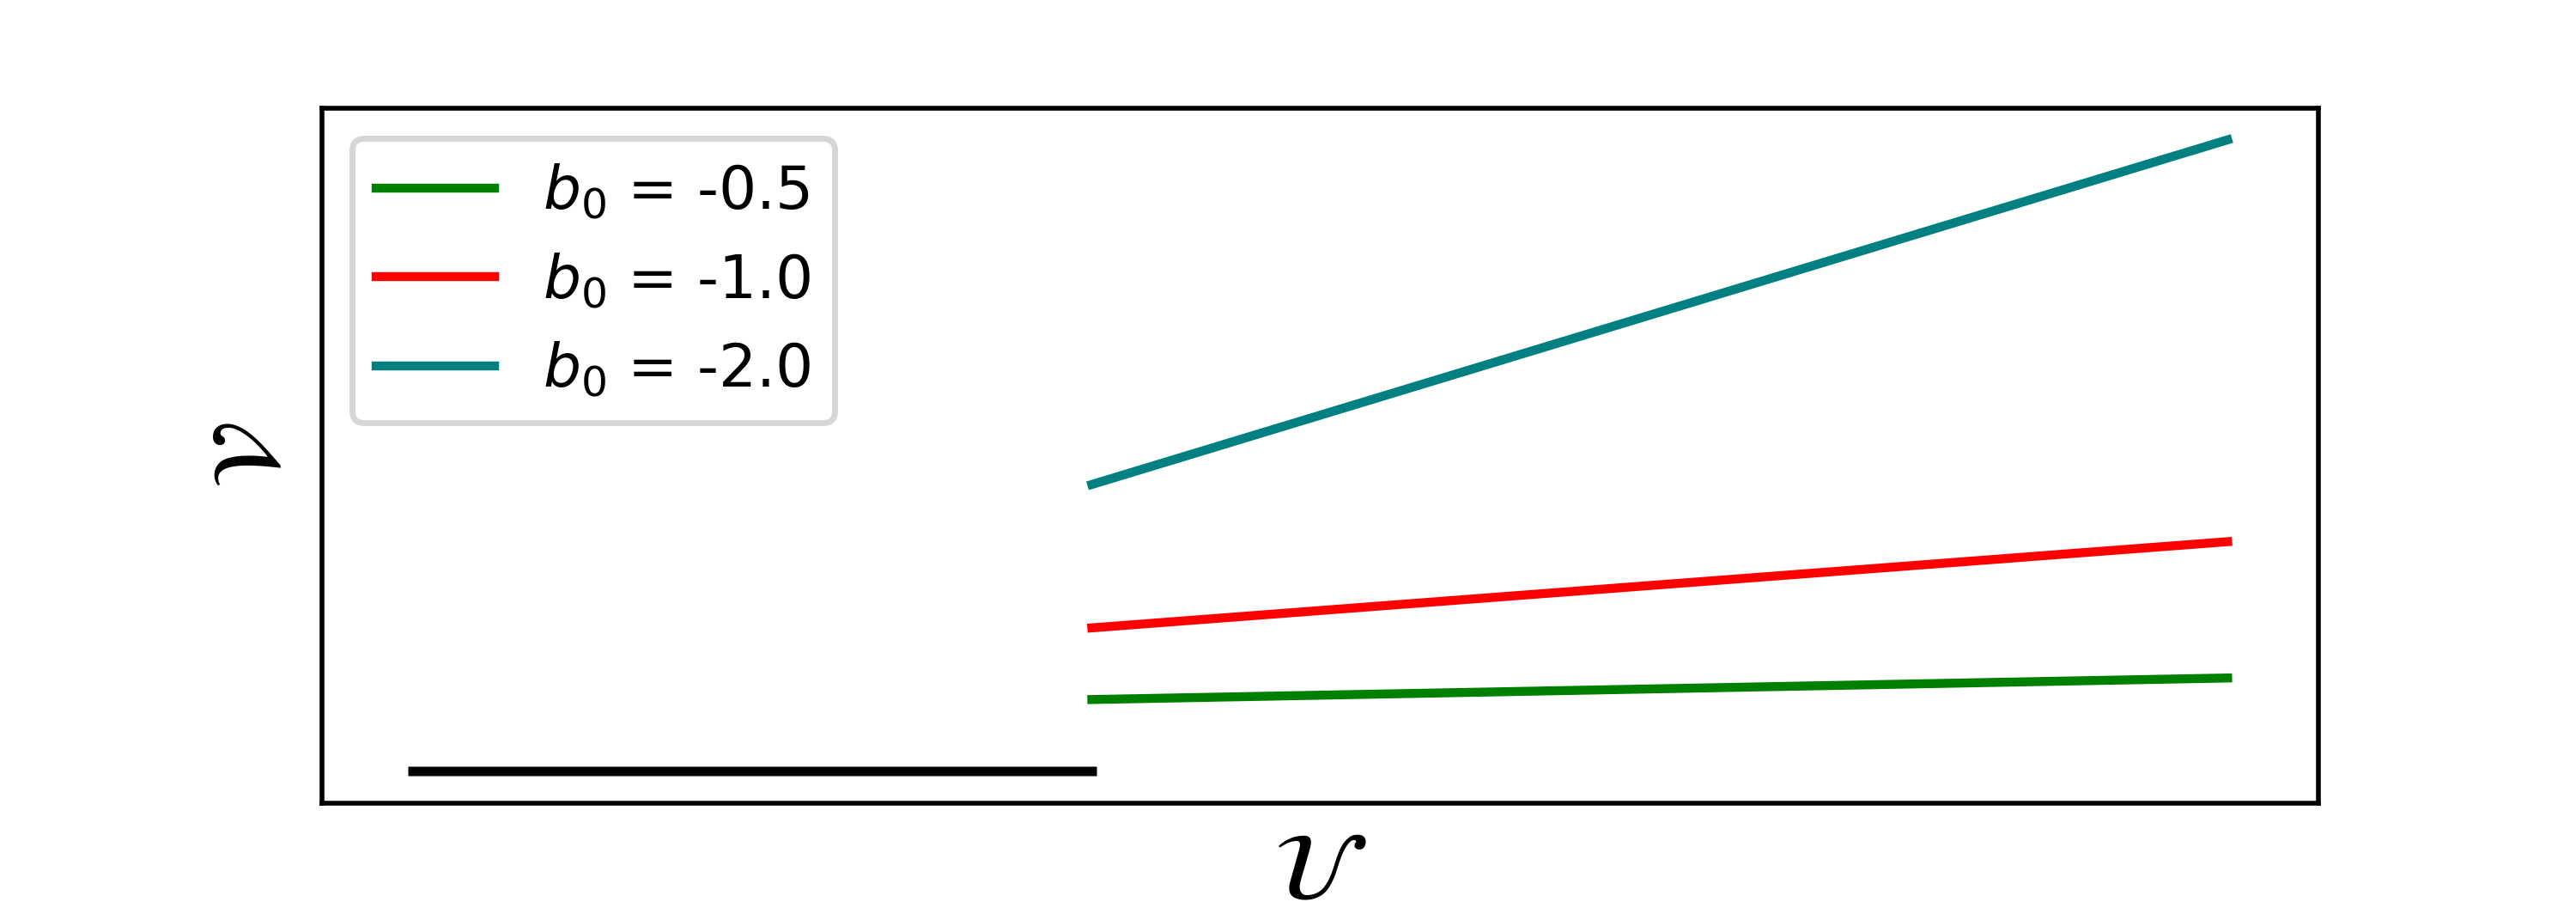
\includegraphics[width=.95\textwidth, clip]{../img/kap02/ASNullRing_UV.png}};
    \end{tikzpicture}
     \caption{Nulové geodetiky ($\dot \matu^-=1$, $\dot \matv^-=0$, $\dot \eta^-=0$) procházející impulsem
     Aichelburg-Sexlova řešení v $\rho=2$ pro různé parametry $b_0$.}
     \label{fig:Null_UV_AichelburgSexl_parameters}
\end{figure}

Na obrázku \ref{fig:Null_UV_AichelburgSexl_parameters} je vyobrazena refrakce v Aichelburg-Sexlově řešneí pro různé
parametry $b_0$. Dochází ke skoku v souřadnici $\matv$, jak plyne z Penroseových napojovacích podmínek, a k refrakci.
S rostoucí absolutní hodnotou parametru $b_0$ dochází k větší změně ve složce rychlosti $\dot \matv$.
Skok ve složce $\dot \matv$ doprovází změna ve složce $\dot \eta$, pro kterou opět platí, že se spolu s
rostoucí absolutní hodnotou $b_0$ dochází k větší změně. Tato závislost je také vidět na obrázku \ref{fig:NullASRing01},
kde vidíme geodetikcý pohyb v prostoru v závislosti na retardované souřadnici $\matu$, kterou v případě neexpandujících vln
v Minkowského prostoročase můžeme použít jako afinní parametr.

\begin{figure}[h]
    \centering
    \begin{subfigure}[b]{0.45\textwidth}
        \begin{tikzpicture}
            \node[inner sep=0pt, anchor=south west] (ds) at (0,0)
        {\adjincludegraphics[trim={{.1\width} {.15\height} {.1\width} {.25\height}}, width=\textwidth, clip]{../img/kap02/ASNullRingxyUmu-1.pdf}};
        \filldraw[white] (0.59,2.65) circle (5pt);
        \node[text width=7pt] at (0.59,2.65) {\footnotesize{$\matu$}};
        \end{tikzpicture}
        \caption{$b_0 = -1$}
    \end{subfigure}
    \hfill
    \begin{subfigure}[b]{0.45\textwidth}
        \begin{tikzpicture}
            \node[inner sep=0pt, anchor=south west] (ds) at (0,0)
            {\adjincludegraphics[trim={{.1\width} {.15\height} {.1\width} {.25\height}}, width=\textwidth, clip]{../img/kap02/ASNullRingxyUmu-2.pdf}};
            \filldraw[white] (0.59,2.65) circle (5pt);
            \node[text width=7pt] at (0.59,2.65) {\footnotesize{$\matu$}};
        \end{tikzpicture}
        \caption{$b_0 = -2$}
    \end{subfigure}
    \caption{Nulové geodetiky ($\dot \matu^-=1$, $\dot \matv^-=0$, $\dot \eta^-=0$) procházející impulsní vlnou Aichelburg-Sexlova řešení. Prstenec testovacích částic je před průchodem impulsem v $\rho=2$.}
    \label{fig:NullASRing01}
\end{figure}

Záporné hodnoty parametru $b_0$, použté na obrázcích \ref{fig:Null_UV_AichelburgSexl_parameters} a \ref{fig:NullASRing01}, byly vhodné pro přehlednější vizualizaci
efektu impulsní vlny, nemají ale v originální konstrukci Aichelburg-Sexlova ultraboostu fyzikální význam. Parametr $b_0$
představuje v ultraboostové limitě $v \to 1, m \to 0$ konstantu, která splňuje $8m = b_0\sqrt{1-v^2}$, pro fyzikální systémy konstruované touto metodou
tedy nabývá kladných hodnot. Příklady nulových geodetiky pro tyto hodnoty jsou na obrázku \ref{fig:ASNullFyzikalnejsi}, vidíme,
že geodetiky jsou refraktovány směrem k $\rho=0$ -- jde tedy o přitažlivý efekt nulové částice generující impulsní vlnu.

\textcolor{red}{Jak moc vadí, že ty geodetiky jdou vlastně pozpátku v souřadnicovém čase??}


\begin{figure}[ht]
    \centering
    \begin{subfigure}[b]{0.45\textwidth}
        \begin{tikzpicture}
            \node[inner sep=0pt, anchor=south west] (ds) at (0,0)
            {\adjincludegraphics[trim={{.1\width} {.1\height} {.1\width} {.25\height}}, width=\textwidth, clip]{../img/kap02/ASNullRingxyUmu1.pdf}};
            \filldraw[white] (0.59,3.1) circle (5pt);
            \node[text width=7pt] at (0.59,3.1) {\footnotesize{$\matu$}};
        \end{tikzpicture}
        \caption{$b_0 = 1$}
    \end{subfigure}
    \hfill
    \begin{subfigure}[b]{0.45\textwidth}
        \begin{tikzpicture}
            \node[inner sep=0pt, anchor=south west] (ds) at (0,0)
            {\adjincludegraphics[trim={{.1\width} {.1\height} {.1\width} {.25\height}}, width=\textwidth, clip]{../img/kap02/ASNullRingxyUmu2.pdf}};
            \filldraw[white] (0.59,3.1) circle (5pt);
            \node[text width=7pt] at (0.59,3.1) {\footnotesize{$\matu$}};
        \end{tikzpicture}
        \caption{$b_0 = 2$}
    \end{subfigure}
\caption{Nulové geodetiky ($\dot \matu^-=1$, $\dot \matv^-=0$, $\dot \eta^-=0$) procházející impulsem v $\rho=2$ pro kladné hodnoty parametru $b_0$.}
\label{fig:ASNullFyzikalnejsi}
\end{figure}

Testovací částice na časupodobných geodetikách se chovají stejným způsobem, na obrázku \ref{fig:AsMatter01} vidíme časupodobné geodetiky,
po kterých se testovací částice šíří paralelně s osou $z$. Při průchodu $\matu = 0$ dojde k refrakci a částice po průchodu letí směrem k ose $z$.

\begin{figure}[ht]
    \centering
    \begin{subfigure}[b]{0.45\textwidth}
        \begin{tikzpicture}
            \node[inner sep=0pt, anchor=south west] (ds) at (0,0)
        {\adjincludegraphics[trim={{.1\width} {.15\height} {.1\width} {.25\height}}, width=\textwidth, clip]{../img/kap02/ASMatterRingxyUmu0.5.pdf}};
        \filldraw[white] (0.59,2.6) circle (5pt);
        \node[text width=7pt] at (0.59,2.6) {\footnotesize{$\matu$}};
        \end{tikzpicture}
        \caption{$b_0 = 0.5$}
    \end{subfigure}
    \hfill
    \begin{subfigure}[b]{0.45\textwidth}
        \begin{tikzpicture}
            \node[inner sep=0pt, anchor=south west] (ds) at (0,0)
            {\adjincludegraphics[trim={{.1\width} {.15\height} {.1\width} {.25\height}}, width=\textwidth, clip]{../img/kap02/ASMatterRingxyUmu2.pdf}};
            \filldraw[white] (0.59,2.6) circle (5pt);
            \node[text width=7pt] at (0.59,2.6) {\footnotesize{$\matu$}};
        \end{tikzpicture}
        \caption{$b_0 = 2$}
    \end{subfigure}
    \caption{Časupodobné geodetiky ($\dot \matu^-=\frac{1}{2}$, $\dot \matv^-=1$, $\dot \eta^-=0$) procházející impulsní vlnou AS řešení. Prstenec testovacích částic je před průchodem impulsem v $\rho=2$.}
    \label{fig:AsMatter01}
\end{figure}

Refrakce je slabší s rostoucí vzdáleností od částice generující impuls. Na obrázku \ref{fig:AS_zavislost_na_rho} jsou znázorněny už
refraktované časupodobné geodetiky pro různé vzdálenosti od osy symetrie. Před refrakcí se jedná o pohyb testovacích částic ve směru osy $z$.

\begin{figure}[!ht]
    \centering
       \begin{tikzpicture}
           \node[inner sep=0pt, anchor=south west] (ds) at (0,0)
           {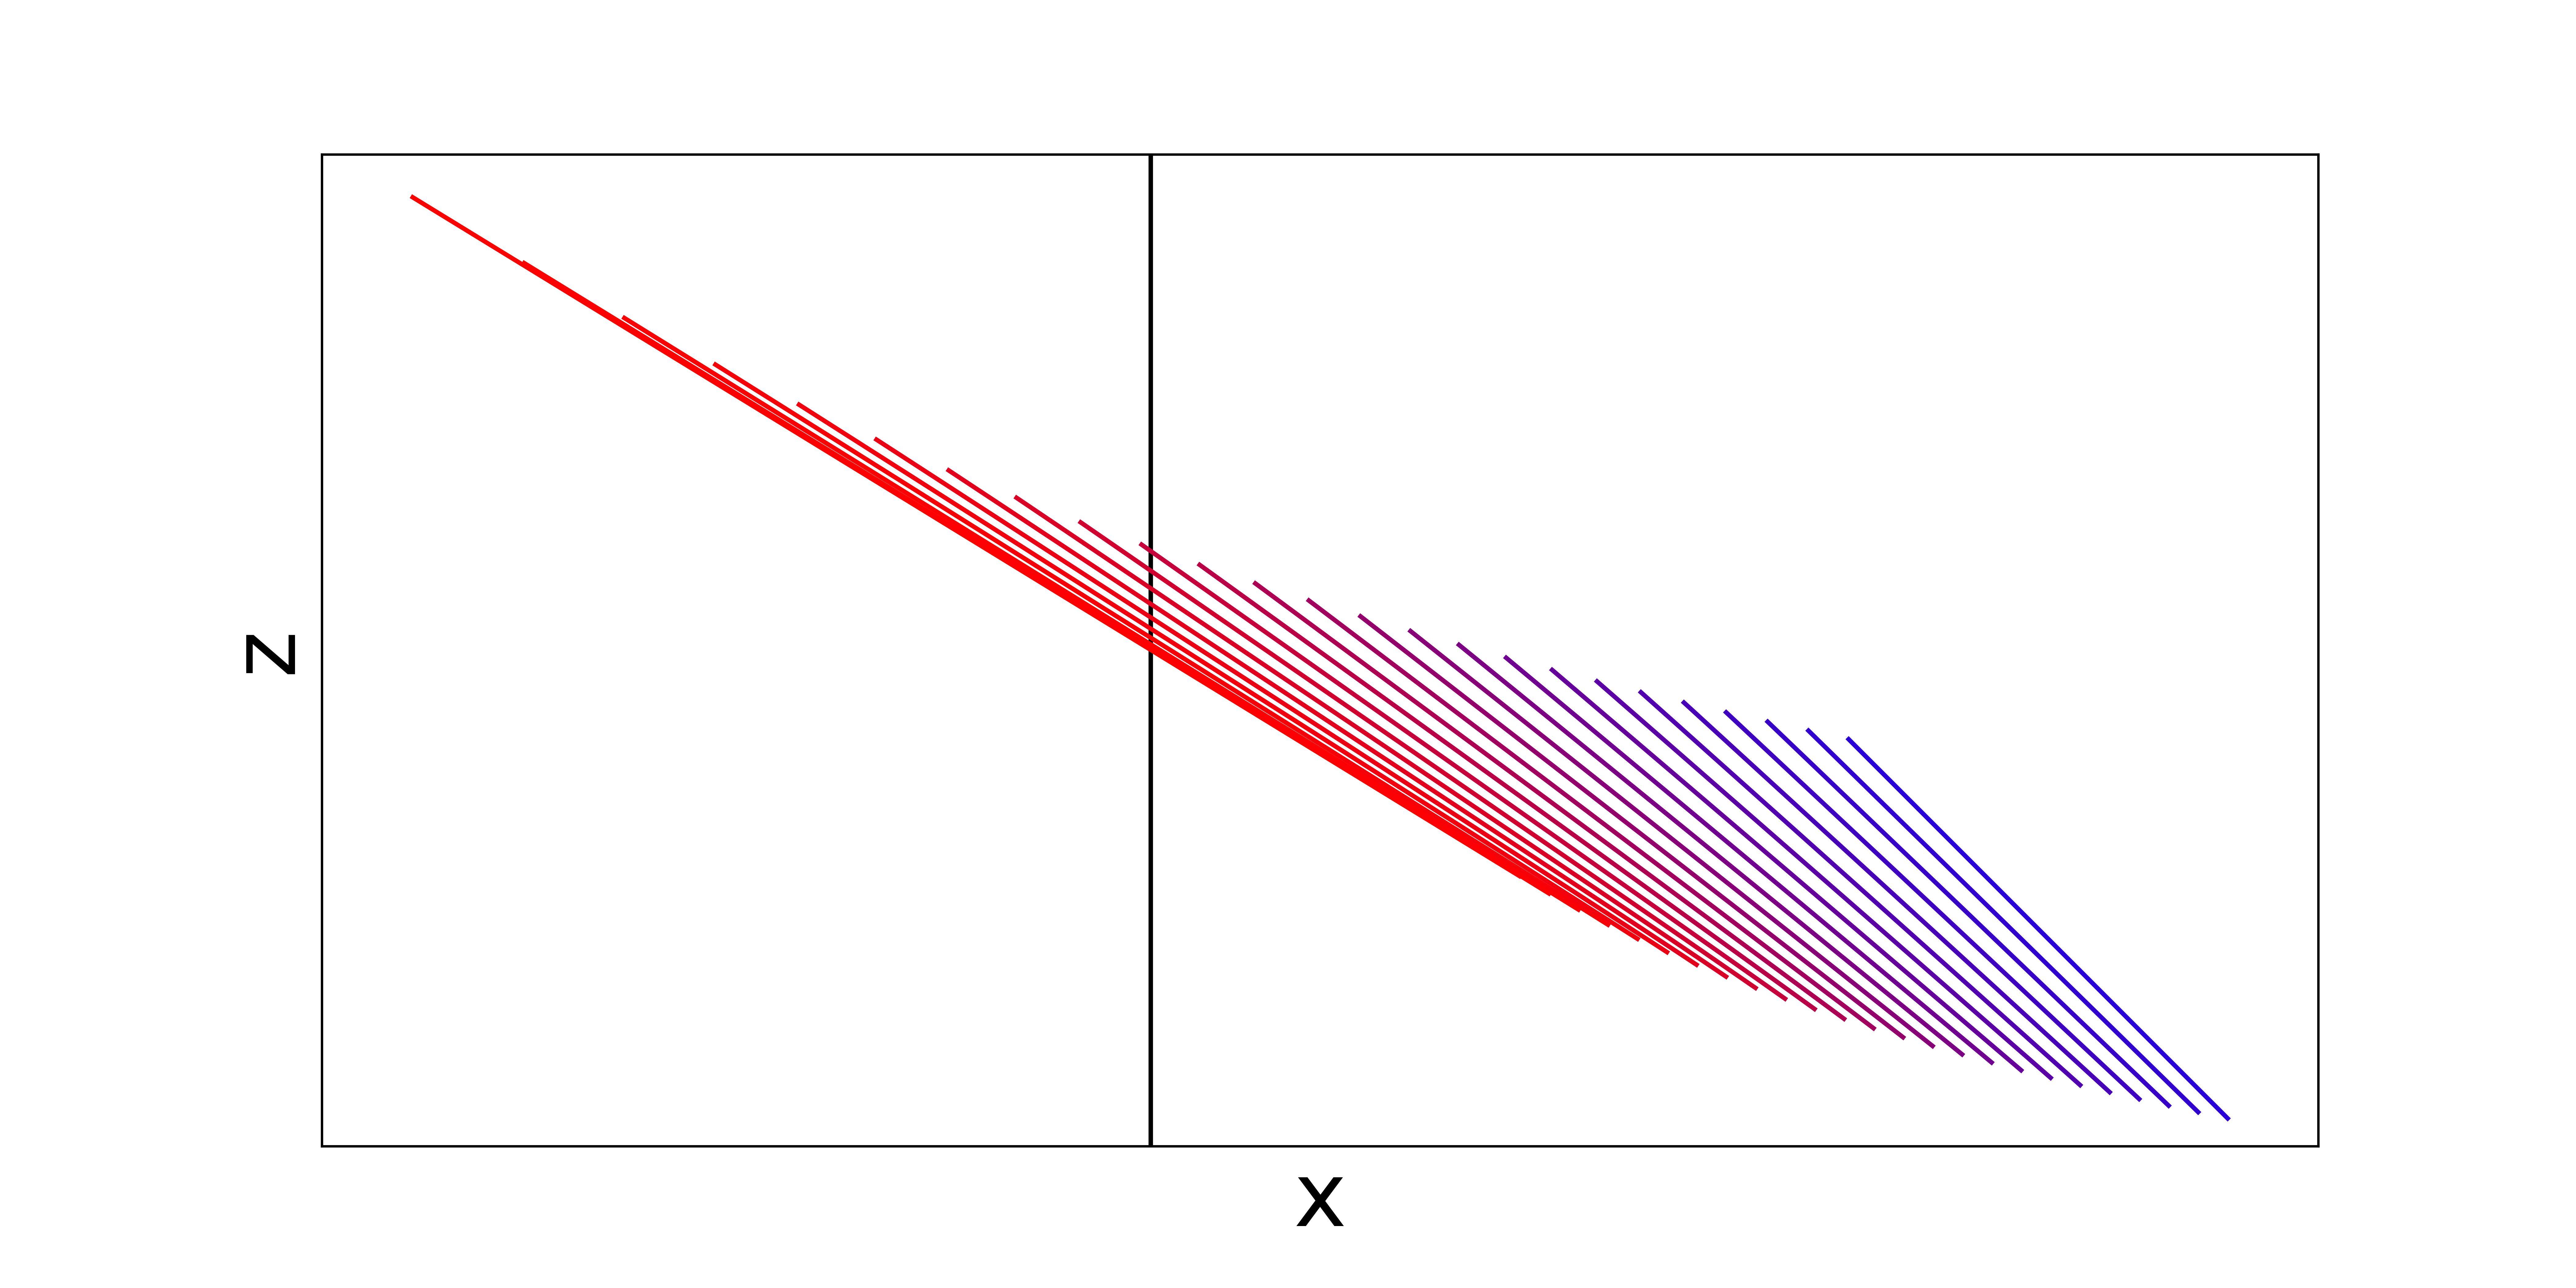
\includegraphics[width=.7\textwidth, clip]{../img/kap02/ASMatterLinexz.png}};
        \end{tikzpicture}
    \caption{Refraktované časupodobné geodetiky po průchodu impulsem v různých vzdálenostech $\rho$ pro $b_0 = \frac{1}{2}$.
    Červená barva odpovídá částici refraktované nejblíže ($\rho=\frac{1}{2}$), modrá nejdále ($\rho = 2$). Černá přímka odpovídá
    ose $x=0$.}
    \label{fig:AS_zavislost_na_rho}
\end{figure}


Pro potěšení oka čtenáře jsou přiloženy další vizualizace geodetického pohybu v Aichelburg-Sexlově řešní. Na obrázku \ref{fig:AsMatter02} se jedná systém časupodobných geodetik, které se před
průchodem impulsní vlnou šíří od osy symetrie $z$. V (b) dochází k refrakci, která otáčí směr šíření směrem zpět k ose $z$.
Na obrázku \ref{fig:AsMatterNonAxial} je pak zobrazení průchodu geodetik, které nejsou uspořádáný axiálně symetricky.

\begin{figure}[ht]
    \centering
    \begin{subfigure}[b]{0.45\textwidth}
        \begin{tikzpicture}
            \node[inner sep=0pt, anchor=south west] (ds) at (0,0)
        {\adjincludegraphics[trim={{.1\width} {.15\height} {.1\width} {.25\height}}, width=\textwidth, clip]{../img/kap02/ASMatterRing_XYMOVING__xyU_mu2.pdf}};
        \filldraw[white] (0.59,2.7) circle (5pt);
        \node[text width=7pt] at (0.59,2.7) {\footnotesize{$\matu$}};
        \end{tikzpicture}
        \caption{$b_0 = 2$}
    \end{subfigure}
    \hfill
    \begin{subfigure}[b]{0.45\textwidth}
        \begin{tikzpicture}
            \node[inner sep=0pt, anchor=south west] (ds) at (0,0)
            {\adjincludegraphics[trim={{.1\width} {.15\height} {.1\width} {.25\height}}, width=\textwidth, clip]{../img/kap02/ASMatterRing_XYMOVING__xyU_mu4.pdf}};
            \filldraw[white] (0.59,2.7) circle (5pt);
            \node[text width=7pt] at (0.59,2.7) {\footnotesize{$\matu$}};
        \end{tikzpicture}
        \caption{$b_0 = 4$}
    \end{subfigure}
    \caption{Časupodobné geodetiky ($\dot \matu^-=1$, $\dot \matv^-=2$, $\dot \eta^-=\sqrt{\frac{3}{2}} e^{i \phi}$), kde $\phi$ odpovídá úhlu v
    cylindrických souřadnicích ve kterém částice leží, procházející impulsní vlnou AS řešení v $\rho=2$.}
    \label{fig:AsMatter02}
\end{figure}

\begin{figure}[ht]
    \centering
    \begin{tikzpicture}
        \node[inner sep=0pt, anchor=south west] (ds) at (0,0)
        {\adjincludegraphics[trim={{.1\width} {.15\height} {.1\width} {.22\height}}, width=0.8\textwidth, clip]{../img/kap02/ASMatterHearthxyUmu1.pdf}};
        \filldraw[white] (1.87,2.7) circle (9pt);
        \node[text width=9pt] at (1.87,2.7) {\small{$\matu$}};
    \end{tikzpicture}    
    \caption{Časupodobné geodetiky ($\dot \matu^-=\frac{1}{2}$, $\dot \matv^-=1$, $\dot \eta^-=0$) ve vybraném uspořádání, procházející nadplochou $\matu = 0$.}
    \label{fig:AsMatterNonAxial}
\end{figure}
Pro $m>0$ závisí změna geodetického pohybu na prostorovém úhlu. Derivace $H_{i,Z}$m která vystupuje v refrakčních rovnicíchm je pro jednotlivá $m$
\begin{equation}
    H_{i,Z}^{(m)}(\eta, \bar{\eta}) = -\frac{(\sqrt{2})^{m} b_m m}{\eta^{m+1}}.
\end{equation}
Speciálně pro $m=1$, tedy impuls generovaný částicí s dipólovou strukturou, je vykreslena na obrázku \ref{fig:DipoleHZ}. \textcolor{red}{Tento obrázek mi příjde trochu nicneříkající, bez hlubšího zamyšlení,
možná odstranit nebo popsat (což bude vyžadovat právě to hlubší zamyšlení).}

Příklad nulových geodetik procházejících impulsem s jediným nenulovým členem pro $m=1$ je na obrázku \ref{fig:DipoleHZ}

\begin{figure}[ht]
    \centering
    \begin{subfigure}[b]{0.45\textwidth}
        \begin{tikzpicture}
            \node[inner sep=0pt, anchor=south west] (ds) at (0,0)
        {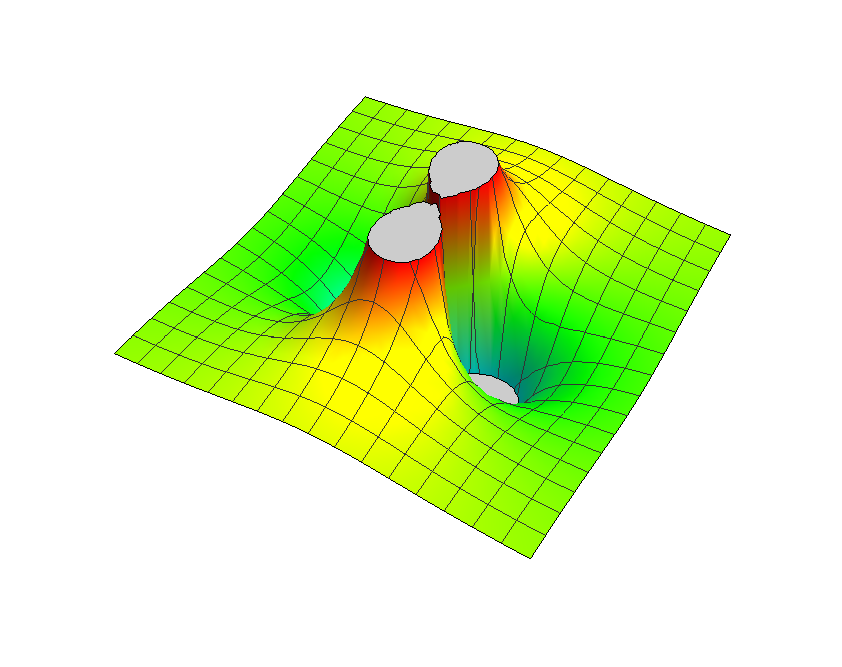
\includegraphics[width=1\textwidth, clip]{../img/kap02/DipoleHZReal.pdf}};
        \end{tikzpicture}
        \caption{$Re(H_{i,Z}^{(1)})$}
    \end{subfigure}
    \hfill
    \begin{subfigure}[b]{0.45\textwidth}
        \begin{tikzpicture}
            \node[inner sep=0pt, anchor=south west] (ds) at (0,0)
            {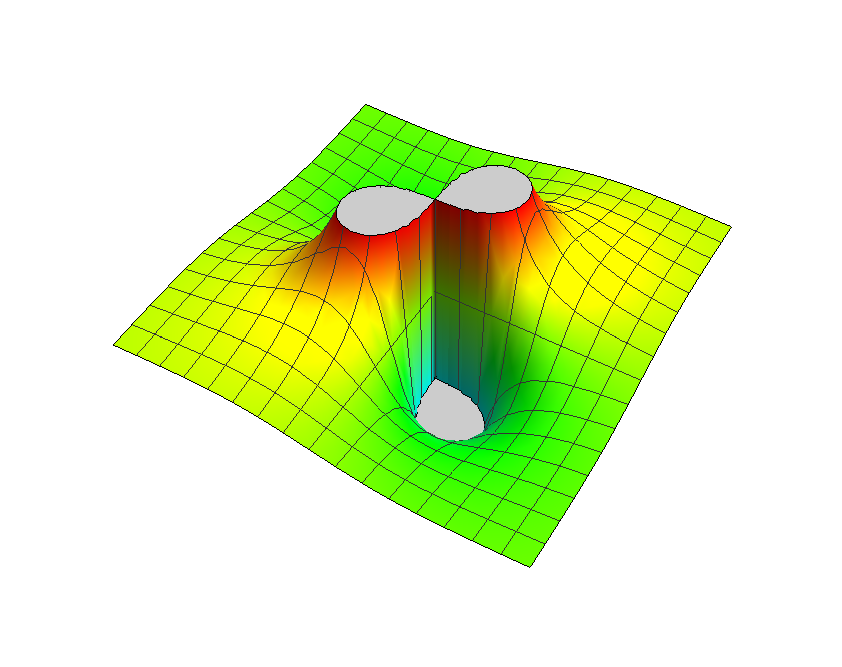
\includegraphics[width=1\textwidth, clip]{../img/kap02/DipoleHZImaginary.pdf}};
        \end{tikzpicture}
        \caption{$Im(H_{i,Z}^{(1)})$}
    \end{subfigure}
    \caption{Reálná a imaginární část $H_{i,Z}^{(1)}(x, y)$.}
    \label{fig:DipoleHZ}
\end{figure}
\begin{figure}[ht]
    \centering
    \begin{tikzpicture}
        \node[inner sep=0pt, anchor=south west] (ds) at (0,0)
        {\adjincludegraphics[trim={{.1\width} {.15\height} {.1\width} {.22\height}}, width=0.8\textwidth, clip]{../img/kap02/DipoleNullxyUb1_0.2.pdf}};
        \filldraw[white] (9.1,2) circle (9pt);
        \node[text width=9pt] at (9.1,2) {\small{$\matu$}};
    \end{tikzpicture}    
    \caption{Nulové geodetiky ($\dot \matu^-=1$, $\dot \matv^-=0$, $\dot \eta^-=0$) ve axiálně symetrickém uspořádání ($\rho=1$), procházející impulsní nadplochou vlny generované částicí s dipólovou strukturou,
    s parametrem $b_1=0.2$.}
    \label{fig:DipoleAxial}
\end{figure}
\clearpage

\subsection{Impulsní gravitační vlna generovaná nehmotnými částicemi s multipólovou strukturou s $\Lambda\neq 0$}

V prostoročasech s nenulovou konstantou odvodili Griffiths a Podolský \cite{Podolsky1997} tvar řešení obdobný \eqref{eq:multipole_minkowski},
tedy impulsních vln generovaných nulovými částicemi s multipólovou strukturou. Vyšli z redukce Einsteinových rovnic pro distribuční
metriku \eqref{eq:5DDistributionalWaveMetric}. V případě ryze gravitačních vln dostáváme podmínku

\begin{equation}
    \label{eq:podminka_na_H_lambda_stare}
    \left(\Delta + \frac{2}{3} \Lambda \right)\mathcal{H} = 0,
\end{equation}

kde $\Delta$ je laplaceův operátor působící na impulsní nadploše. Při parametrizaci 

\begin{equation}
    \begin{split}
        Z_2 &= a \sqrt{\epsilon(1-z^2)} \cos \phi\\
        Z_3 &= a \sqrt{\epsilon(1-z^2)} \sin \phi\\
        Z_4 &= a~z
    \end{split}
\end{equation}

nabývá funkce $\mathcal{H}(z, \phi)$ tvaru
\begin{equation}
    \mathcal{H}(z, \phi) = b_0 Q_1(z) + \sum_{m=1}^\infty b_0 Q_1^m(z) \cos [m(\phi - \phi_m)],
\end{equation}

kde $Q_1^m(z)$ jsou přidružené Legendrovy funkce druhého druhu
\begin{equation}
    Q_1^m(z) = -(\epsilon)^m |1-z^2|^{m/2} \frac{d^m}{dz^m}Q_1(z)
\end{equation}

První člen
\begin{equation}
    b_0 Q_1(z) = b_0 \frac{z}{2} \log \left|\frac{1+z}{1-z}\right| - 1
\end{equation}
představuje axiálně symetrické Hottovo-Tanakovo řešení \cite{Hotta_1993}, které odpovídá boostu Schwarzschildova-(anti-)de Sitterova
prostoročasu, jde o analogii Aichelburg-Sexlova řešení v (anti-)de Sitterově prostoročasu. V případě de Sitterova prostoročasu je impulsní nadplocha
neexpandující sféra generovaná dvěma nehmotnými částicemi které letí v opačném směru. V anti-de Sitterové prostoročasu je impulsní plochou nadplocha hyperboloidální
plochou, generovanou částicí, která se (díky díky tomu, že se jedná o nakrytí $\mathbb{R}^4$ s topologií $\mathbb{S^1} \times \mathbb{R}^3$) periodicky pohybuje mezi prostorovými nekonečny,
z jedné strany na druhou.



